We've presented different dynamical models of the central region of J1331, some of them capturing the observed kinematics well, but none of them work both at small and large radii. In the following we will discuss possible reasons for these deviations, also by comparing our results to previous work.

\subsection{On J1331's stellar mass-to-light ratio} \label{sec:MLdiscussion}

Further knowledge of the stellar populations within J1331 and their initial mass functions (IMF) would be useful. In particular a sophisticated guess for the \emph{stellar} mass-to-light ratio in J1331's bulge could be compared to our very reliable measurement of the \emph{total} mass-to-light ratio inside the Einstein radius (see Table \ref{tab:einsteinML} ) to support or contradict the presence of a significant amount of dark matter in the bulge.

Traditional choices for the IMF are the bottom-heavy IMF by \citet{Salpeter1955},
$$\xi(m) \propto m^{-x}, x=2.35,$$
where $\xi(m) \diff m$ is the number of stars with mass $m$ in $[m,m+\diff m]$, and the IMFs by \citet{2002Sci...295...82K} and \citet{Chabrier2003}, which are in agreement with each other and predict less low-mass stars.

\citet{Ferreras} found a relation between the central stellar velocity dispersion $\sigma_0$ in early-type galaxies and the IMF slope. A higher $\sigma_0$ suggests a more bottom-heavy IMF. For an unimodal (Salpeter-like) IMF and a $\sigma_0 \simeq 200~\text{km s}^{-1}$ for J1331 (see Figure \ref{fig:kinematics}) they predict $x \approx 2.33$, which is close to the standard Salpeter slope, also supported by \citet{2014MNRAS.438.1483S}. When assuming a bi-modal (Kroupa-equivalent-like) IMF, \citet{Ferreras} predict $x \approx 2.85$ for J1331's central velocity dispersion. This is more bottom-heavy than the standard \citet{2002Sci...295...82K} IMF. Overall the central velocity dispersion suggests a rather bottom-heavy IMF J1331's bulge and therefore large stellar mass-to-light ratio. \citet{SWELLSI} estimated J1331's stellar bulge mass given a Salpeter IMF and measured the I-band AB magnitude of the bulge. Transformed to a stellar I-band mass-to-light ratio (see Table \ref{tab:previousresults}) this would correspond to $\Upsilon_\text{I,*}^\text{sal} = 4.7 \pm 1.2$.

We compare our findings of the stellar mass-to-light ratios with the study by \cite{SWELLSV}: They found that the bulge of J1331 has an IMF more bottom-heavy than the Salpeter IMF from fitting a NFW halo to (1) the Einstein mass and (2) gas kinematics at larger radii $\gtrsim 8''$. In Section \ref{sec:results_JAM_NFW} we fitted the stellar kinematics within $\sim 3.5''$ and the Einstein mass with a NFW halo and the best fit $\Upsilon_\text{I,*} = 4.2 \pm 0.2$ (see Table \ref{tab:modelB4_bestfit}) indicates a less bottom-heavy IMF than the Salpeter IMF. \cite{SWELLSV}  found systematically lower NFW halos ($v_\text{circ}(5'') \sim 120~\text{km s}^{-1}$ according to their Figure 2) than we did ($v_\text{circ}(5'') \sim 200~\text{km s}^{-1}$, see Figure \ref{fig:kinematics}).

%==============
\begin{figure}
\centering
  \includegraphics[width=0.9\linewidth]{fig/B4_jam_profiles_errors_short_vcirc.ps}
  \caption{Circular velocity curve. \Wilma{[TO DO: Write caption]}}
  \label{fig:modelB4_vcirc}
\end{figure}
%==============

We note however, that our results would be much closer to those by \citet{SWELLSV}, if we only used the lensing results at small radii as they did: The total mass-to-light ratio of $\Upsilon_\text{I,tot}^\text{ein} = 5.6$ inside the Einstein radius (see Table \ref{tab:einsteinML}). In case of a lower mass dark matter halo, the largest contribution to this mass-to-light ratio would then be stellar mass, so that the corresponding IMF would be more bottom-heavy than Salpeter. The circular velocity curve that \citet{SWELLSV} find for J1331 peaks at $v_\text{circ}(R\sim0.9'') \sim 350~\text{km s}^{-1}$ (from lensing constraints only) and at $v_\text{circ}(R\sim0.9'') \sim 370~\text{km s}^{-1}$ (when including a dark matter halo and gas kinematics in the fit). We get a very similar circular velocity curve (at least at small radii) for a mass-follows-light model with constant $\Upsilon_\text{I,tot}^\text{ein} = 5.6$, which peaks at $v_\text{circ}(R\sim0.9'') \sim 360~\text{km s}^{-1}$. From this comparison follows, that the model by \citet{SWELLSV} corresponds approximately to a mass-follows-light model in the inner regions of J1331. In Section \ref{sec:results_JAM_SB} however we showed, that this is \emph{not} a good model for J1331 and won't be able to reproduce the central stellar $v_\text{rms}$ dip. 

On the other hand, because our NFW JAM models fail to predict the stellar kinematics at large radii, the true halo parameters are more likely closer to the findings by \citet{SWELLSV}. All of this leaves the central dip unexplained: It cannot be due to tangential velocity anisotropy in the center alone (see Section \ref{sec:results_JAM_SB}, Figure \ref{fig:JAM_modelA2}). It also cannot be explained by a strong contribution of dark matter inside the bulge together with a moderate tagential velocity anisotropy, because the corresponding dark matter halos would still be too massive to fit the data in the outer regions (see Section \ref{sec:results_JAM_NFW}, Figure \ref{fig:modelB4_vrms}]).

An alternative JAM model was introduced in Section \ref{sec:results_JAM_SB}, where we used the surface brightness distribution without a halo component but together with an increasing mass-to-light ratio. We found that such a model would be perfectly consistent with the lensing results and predict a total mass-to-light ratio in the center of J1331 of  $\Upsilon_\text{I,tot}(R'\sim0) = 2.53$. This is very close to the stellar mass-to-light ratio we got from \citet{SWELLSI} estimates of the bulge's stellar mass using the Chabrier IMF $\Upsilon_\text{I,*}^\text{Chabrier} = 2.5 \pm 0.6$, i.e., less bottom-heavy (more bluish) population.

Another feature in the stellar kinematics, that none of our JAM models was able to reproduce in the slightest and which we therefore excluded in the modelling, was the dip in $v_\text{rms}$ around $\sim 6''$, which occurs around the transition from bulge to disk (see Figures \ref{fig:F814W} and \ref{fig:kinematics}).

The above discussion motivates the following speculation: In the absence of a strong dark matter contribution in the center, the overall stellar-mass-to-light ratio within the Einstein radius indicates a bottom-heavy IMF close to the Salpeter IMF, consistent with estimates from the velocity dispersion. At the same time the central dip can then be only explained, if there was an increase in stellar mass-to-light ratio with radius \textit{within} the bulge. \emph{If} there was a central stellar population with an IMF close to the \citet{Chabrier2003} IMF, surrounded by a more bottom-heavy population, the central stellar kinematics would be well explained and be fully consistent with the lensing results. (According to Figure \ref{fig:lenscompareboth} the lensing result might not predict a mass to light ratio gradient inside $R_\text{ein}$, but then again the mass slope $alpha=1$ was only weakly constrained.) The disk of J1331 has a lower $\Upsilon_\text{I,*}$ than the bulge (see Table \ref{tab:previousresults} according to \citet{SWELLSI}). Such a drop in $\Upsilon_\text{I,*}$ at the transition region from bulge to disk around $\sim 5''$ could lead to the observed drop in $v_\text{rms}$, while an increasing contribution of a lower mass dark matter halo at larger radii as found by \citet{SWELLSV}, would recover the kinematics in the out regions of J1331's disk.

\Wilma{[TO DO: Why are disk and bulge mass in SWELLS I different to the one in SWELLS IV??]}

\begin{table*}
\centering
\begin{tabular}{cccccc}
\hline\hline
& & \multicolumn{2}{c}{Chabrier IMF} & \multicolumn{2}{c}{Salpeter IMF}\\
      &  $L$ [$10^{10}L_{\odot}$]                & $M_*$ [$10^{10}M_\odot$]               & $\Upsilon_\text{I,*}^\text{chab}$ & $M_*$ [$10^{10}M_\odot$] & $\Upsilon_\text{I,*}^\text{sal}$ \\\hline
bulge &   $3.10 \pm 0.15 $  & $7.8 \pm 1.8$ & $2.5 \pm 0.6$ & $14.5 \pm 3.7 $ & $4.7 \pm 1.2$ \\
disk  &   $2.35 \pm 0.11 $  & $2.9 \pm 0.7$ & $1.2 \pm 0.3$ & $5.2 \pm 1.1$ & $2.2 \pm 0.5$ \\
total &   $5.45 \pm 0.19$ & $10.6 \pm 1.9$& & $19.7 \pm 3.9$&\\\hline
\end{tabular}
\caption{Total I-band luminosity, stellar mass and mass-to-light ratio, calculated from the I-band AB magnitudes and stellar masses found for J133's bulge and disk by \citet{SWELLSI} (their table 2) for comparison with this work. The transformation from AB magnitudes to the Johnson-Cousins I-Band used the relation $I[\text{mag}] = I[\text{ABmag}] - 0.309$ from \citet{FG1994} (their table 2). For the conversion from apparent magnitude to total luminosity the redshift $z=0.113$ \citet{SWELLSIII} was turned into a luminosity distance using the cosmology by \citet{WMAP5cosm}. }
\label{tab:previousresults}
\end{table*}